\documentclass{ctexart}
% 此处引入常用包,从此行到46行均无需修改
\usepackage[dvipsnames, svgnames, x11names]{xcolor}
\usepackage{listings}
\usepackage{graphicx}
\usepackage{tabularx}
\usepackage[most]{tcolorbox}
\usepackage{amsmath}
\usepackage{multicol}
\usepackage{multirow}
\usepackage{pifont}
\usepackage{enumitem}
\usepackage{bbding}
\usepackage{colortbl}
\usepackage{placeins}
\usepackage{mathpazo}
\usepackage{bm}
\usepackage{tikz}
\usepackage{xparse}
\usepackage{fancyhdr}
\usepackage[ruled,linesnumbered]{algorithm2e}
\usepackage{algorithmic}
\usepackage{tikz}

%代码环境设置
\lstset{
    numbers = none ,                                    %可选参数有none,right,left
    breaklines ,                                        %换行有影响,不加这个则换行时从头开始
    numberstyle = \tiny ,                               %数字大小’
    keywordstyle = \color{blue!70} ,                    %关键字颜色
    commentstyle =\color{black!40!white} ,              %注释颜色
    frame = shadowbox ,                                 %阴影设置
    rulesepcolor = \color{red!20!green!20!blue!20} ,    %阴影颜色设置
    escapeinside =`',                                   %lst中文支持不太好,可以用这个括在中文旁边
    basicstyle =\footnotesize\ttfamily                  %代码字体设置
}

%定义题目计数器和命令
\newcounter{questioncnt}
\newcounter{subquestioncnt}[questioncnt]
\newcounter{subsubquestioncnt}[subquestioncnt]

\NewDocumentCommand\question{om}{\noindent\IfNoValueTF{#1}{\textcolor{blue}{\stepcounter{questioncnt}\arabic{questioncnt}}}{#1}\quad#2\par}
\NewDocumentCommand\subquestion{om}{\noindent\IfNoValueTF{#1}{\textcolor{blue}{\stepcounter{subquestioncnt}\arabic{questioncnt}.\arabic{subquestioncnt}}}{#1}\quad#2\par}
\NewDocumentCommand\subsubquestion{om}{\noindent\IfNoValueTF{#1}{\textcolor{blue}{\stepcounter{subsubquestioncnt}\arabic{questioncnt}.\arabic{subquestioncnt}.\arabic{subsubquestioncnt}}}{#1}\quad#2\par}

%定义回答计数器和命令
\newcounter{answercnt}
\newcounter{subanswercnt}[answercnt]
\newcounter{subsubanswercnt}[subanswercnt]

\NewDocumentCommand\answer{o}{\noindent\textcolor{blue}{\IfNoValueTF{#1}{\stepcounter{answercnt}\arabic{answercnt}}{#1}}\quad}
\NewDocumentCommand\subanswer{o}{\noindent\textcolor{blue}{\IfNoValueTF{#1}{\stepcounter{subanswercnt}\arabic{answercnt}.\arabic{subanswercnt}}{#1}}\quad}
\NewDocumentCommand\subsubanswer{o}{\noindent\textcolor{blue}{\IfNoValueTF{#1}{\stepcounter{subsubanswercnt}\arabic{answercnt}.\arabic{subanswercnt}.\arabic{subsubanswercnt}}{#1}}\quad}

%在此处进行基本信息修改
\newcommand{\sCourse}{计算机网络}   %课程名
\newcommand{\nTime}{五}             %作业次数
\newcommand{\sName}{黄昊}           %学生姓名
\newcommand{\sNumber}{20204205}     %学号

%页边距设置
\usepackage[left=2cm,right=2cm,top=3cm,bottom=2cm]{geometry}

%页眉页脚设置
\pagestyle{fancy}
\fancyhead[C]{\today}

\newcommand{\homeworkTitle}{
    \setcounter{answercnt}{0}
    %标题部分修改
    \begin{center}
        \fontsize{16pt}{0}{\textbf{\kaishu\sCourse课程\quad第\nTime次作业}}\\
        \fontsize{13pt}{0}{\textit{\kaishu\sName\qquad\sNumber}}\\
    \end{center}}

\begin{document}
    \setcounter{answercnt}{0}
    %标题部分修改
    \begin{center}
        \fontsize{16pt}{0}{\textbf{\kaishu\sCourse课程\quad第\nTime次作业}}\\
        \fontsize{13pt}{0}{\textit{\kaishu\sName\qquad\sNumber}}
    \end{center}

\answer[5-08]
UDP将从应用层接收到的报文加上首部后就直接交付给网络层。而TCP
对应用层交付下来的数据块当作字节流处理,不保证接收方和发送方的数据块
大小一模一样,但能保证字节流完全一样,这就是面向字节流的含义。

\answer[5-17]
不行,会导致发送方一直超时重传,一直传送重复的报文段。

\answer[5-18]
\begin{center}
    

\tikzset{every picture/.style={line width=0.75pt}} %set default line width to 0.75pt        

\begin{tikzpicture}[x=0.75pt,y=0.75pt,yscale=-1,xscale=1]
%uncomment if require: \path (0,428); %set diagram left start at 0, and has height of 428

%Straight Lines [id:da6469713532090215] 
\draw    (250,8.42) -- (251,316.62) ;
%Straight Lines [id:da39948414940102417] 
\draw    (415,10.61) -- (415,315.62) ;
%Straight Lines [id:da3182042766889881] 
\draw    (250.36,62.42) -- (412.39,93.05) ;
\draw [shift={(414.36,93.42)}, rotate = 190.7] [color={rgb, 255:red, 0; green, 0; blue, 0 }  ][line width=0.75]    (10.93,-3.29) .. controls (6.95,-1.4) and (3.31,-0.3) .. (0,0) .. controls (3.31,0.3) and (6.95,1.4) .. (10.93,3.29)   ;
%Straight Lines [id:da17306045923623836] 
\draw    (414.36,93.42) -- (251.95,131.37) ;
\draw [shift={(250,131.82)}, rotate = 346.85] [color={rgb, 255:red, 0; green, 0; blue, 0 }  ][line width=0.75]    (10.93,-3.29) .. controls (6.95,-1.4) and (3.31,-0.3) .. (0,0) .. controls (3.31,0.3) and (6.95,1.4) .. (10.93,3.29)   ;
%Straight Lines [id:da4149247566510297] 
\draw    (250,131.82) -- (412.03,162.45) ;
\draw [shift={(414,162.82)}, rotate = 190.7] [color={rgb, 255:red, 0; green, 0; blue, 0 }  ][line width=0.75]    (10.93,-3.29) .. controls (6.95,-1.4) and (3.31,-0.3) .. (0,0) .. controls (3.31,0.3) and (6.95,1.4) .. (10.93,3.29)   ;
%Straight Lines [id:da029654577132287363] 
\draw    (414,162.82) -- (251.59,200.77) ;
\draw [shift={(249.64,201.23)}, rotate = 346.85] [color={rgb, 255:red, 0; green, 0; blue, 0 }  ][line width=0.75]    (10.93,-3.29) .. controls (6.95,-1.4) and (3.31,-0.3) .. (0,0) .. controls (3.31,0.3) and (6.95,1.4) .. (10.93,3.29)   ;
%Straight Lines [id:da7266936888271076] 
\draw  [dash pattern={on 0.75pt off 0.75pt}]  (249.64,201.23) .. controls (251.73,200.14) and (253.32,200.63) .. (254.41,202.72) .. controls (255.51,204.81) and (257.1,205.3) .. (259.19,204.2) .. controls (261.28,203.11) and (262.87,203.6) .. (263.96,205.69) .. controls (265.05,207.78) and (266.64,208.27) .. (268.73,207.18) .. controls (270.82,206.09) and (272.41,206.58) .. (273.51,208.67) .. controls (274.6,210.76) and (276.19,211.25) .. (278.28,210.16) .. controls (280.37,209.07) and (281.96,209.56) .. (283.05,211.65) .. controls (284.14,213.74) and (285.73,214.23) .. (287.82,213.14) .. controls (289.91,212.05) and (291.5,212.54) .. (292.6,214.63) .. controls (293.69,216.72) and (295.28,217.21) .. (297.37,216.12) -- (299.36,216.74) -- (299.36,216.74) ;
%Curve Lines [id:da7630854567139753] 
\draw  [dash pattern={on 4.5pt off 4.5pt}]  (249.36,27.74) .. controls (299.85,26.75) and (348.38,240.4) .. (410.47,244.68) ;
\draw [shift={(412.36,244.74)}, rotate = 180] [color={rgb, 255:red, 0; green, 0; blue, 0 }  ][line width=0.75]    (10.93,-3.29) .. controls (6.95,-1.4) and (3.31,-0.3) .. (0,0) .. controls (3.31,0.3) and (6.95,1.4) .. (10.93,3.29)   ;
%Straight Lines [id:da8206697881038971] 
\draw    (412.36,244.74) -- (249.95,282.69) ;
\draw [shift={(248,283.14)}, rotate = 346.85] [color={rgb, 255:red, 0; green, 0; blue, 0 }  ][line width=0.75]    (10.93,-3.29) .. controls (6.95,-1.4) and (3.31,-0.3) .. (0,0) .. controls (3.31,0.3) and (6.95,1.4) .. (10.93,3.29)   ;

% Text Node
\draw (245.36,15.4) node  [anchor=north east][inner sep=0.75pt]    {$M_{0}$};
% Text Node 
\draw (245.36,52.4) node  [anchor=north east][inner sep=0.75pt]    {$\mbox{超时重传}M_{0}$};
% Text Node
\draw (245.36,124.4) node [anchor=north east][inner sep=0.75pt]    {$\mbox{发送}M_{1}$};
% Text Node
\draw (245.36,190.4) node [anchor=north east][inner sep=0.75pt]    {$\mbox{发送}M_{0}$};
% Text Node
\draw (245.36,270.4) node [anchor=north east][inner sep=0.75pt]    {$\mbox{收到错误的确认}$};
% Text Node
\draw (418.36,154.4) node [anchor=north west][inner sep=0.75pt]    {$\mbox{收到}M_{1} \mbox{,要求}M_{0}$};
% Text Node
\draw (418.36,234.4) node [anchor=north west][inner sep=0.75pt]    {$\mbox{收到之前超时的}M_{0}$};
% Text Node
\draw (418.36,85.4) node [anchor=north west][inner sep=0.75pt]    {$\mbox{收到}M_{0} \mbox{,要求}M_{1}$};
% Text Node
\draw (300.36,213.4) node [anchor=north west][inner sep=0.75pt]    {$M_{0} \mbox{丢失}$};


\end{tikzpicture}

\end{center}

\answer[5-21]
\subanswer[(1)]
要求收到5,说明5之前的都收到了,但考虑到ACK可能未到达接收方,因此$[5-m,7-m],m\in\{3,2,1,0\}$均有可能。

\subanswer[(2)]
考虑窗口大小,再考虑捎带机制,可以发现2-4都有可能。

\answer[5-22]
\subanswer[(1)]
$2^{32}$个

\subanswer[(2)]
发送帧的个数$N$为$\frac{2^{32}}{1460}$,
总字节数$tot$为$2^{32}+N\times 66$,
所需时间t为$\frac{tot}{1.25MB/s}$,
计算得出时间为3591.3$s$,即 59.85 $min$

\answer[5-27]
65535-20-20=65495字节,其中不考虑可选项字段。

\answer[5-32]
在计算平均往返时间 RTT 时,只要报文段重传了,就不采用其往返时间样本。这就是
Karn算法。

考虑是如何减少的:收到的确认是先发的(就是超时的)而不是超时重发的确认,这一时间会变少。
这一调整导致后面重传的频率越来越频繁,估算的RRT越来越小,进而趋近于0.


\answer[5-35]
传输时延总和:$\frac{960}{48}\times 5 = 100ms$

\quad传播时延总和:$250\times 2 + \frac{1500}{150}\times 3 = 530ms$

\quad总和:$630ms$

\answer[5-36]
$630-20+150=760ms$

\answer[5-39]
\subanswer[(1)]
如下图所示:
\begin{center}
    

\tikzset{every picture/.style={line width=0.75pt}} %set default line width to 0.75pt        

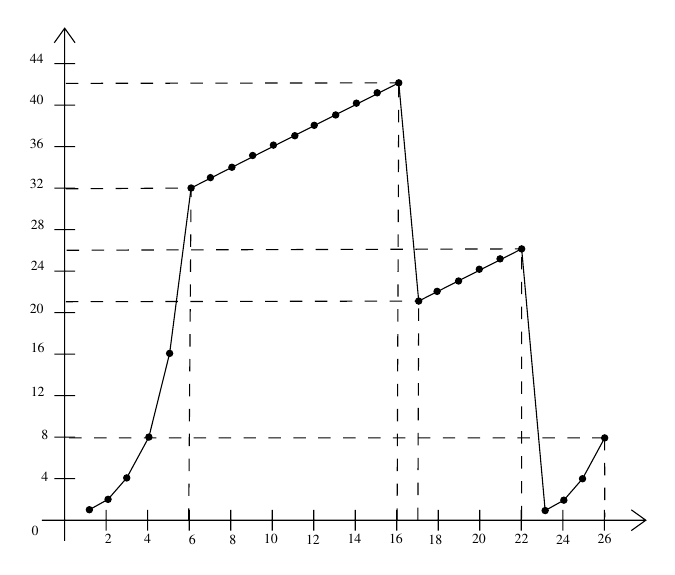
\begin{tikzpicture}[x=0.75pt,y=0.75pt,yscale=-1,xscale=1]
%uncomment if require: \path (0,419); %set diagram left start at 0, and has height of 419

%Shape: Axis 2D [id:dp2295047764388367] 
\draw  (178.56,380.55) -- (469.56,380.55)(189.56,143.52) -- (189.56,390.46) (462.56,375.55) -- (469.56,380.55) -- (462.56,385.55) (184.56,150.52) -- (189.56,143.52) -- (194.56,150.52) (209.56,375.55) -- (209.56,385.55)(229.56,375.55) -- (229.56,385.55)(249.56,375.55) -- (249.56,385.55)(269.56,375.55) -- (269.56,385.55)(289.56,375.55) -- (289.56,385.55)(309.56,375.55) -- (309.56,385.55)(329.56,375.55) -- (329.56,385.55)(349.56,375.55) -- (349.56,385.55)(369.56,375.55) -- (369.56,385.55)(389.56,375.55) -- (389.56,385.55)(409.56,375.55) -- (409.56,385.55)(429.56,375.55) -- (429.56,385.55)(449.56,375.55) -- (449.56,385.55)(184.56,360.55) -- (194.56,360.55)(184.56,340.55) -- (194.56,340.55)(184.56,320.55) -- (194.56,320.55)(184.56,300.55) -- (194.56,300.55)(184.56,280.55) -- (194.56,280.55)(184.56,260.55) -- (194.56,260.55)(184.56,240.55) -- (194.56,240.55)(184.56,220.55) -- (194.56,220.55)(184.56,200.55) -- (194.56,200.55)(184.56,180.55) -- (194.56,180.55)(184.56,160.55) -- (194.56,160.55) ;
\draw   ;
%Straight Lines [id:da7448253421126454] 
\draw    (288.96,204) ;
%Shape: Circle [id:dp4362589907417025] 
\draw  [fill={rgb, 255:red, 0; green, 0; blue, 0 }  ,fill opacity=1 ] (202.96,375.5) .. controls (202.96,374.67) and (202.29,374) .. (201.46,374) .. controls (200.63,374) and (199.96,374.67) .. (199.96,375.5) .. controls (199.96,376.33) and (200.63,377) .. (201.46,377) .. controls (202.29,377) and (202.96,376.33) .. (202.96,375.5) -- cycle ;
%Shape: Circle [id:dp6425396407535877] 
\draw  [fill={rgb, 255:red, 0; green, 0; blue, 0 }  ,fill opacity=1 ] (211.96,370.5) .. controls (211.96,369.67) and (211.29,369) .. (210.46,369) .. controls (209.63,369) and (208.96,369.67) .. (208.96,370.5) .. controls (208.96,371.33) and (209.63,372) .. (210.46,372) .. controls (211.29,372) and (211.96,371.33) .. (211.96,370.5) -- cycle ;
%Shape: Circle [id:dp045670349718068604] 
\draw  [fill={rgb, 255:red, 0; green, 0; blue, 0 }  ,fill opacity=1 ] (220.96,360.17) .. controls (220.96,359.34) and (220.29,358.67) .. (219.46,358.67) .. controls (218.63,358.67) and (217.96,359.34) .. (217.96,360.17) .. controls (217.96,361) and (218.63,361.67) .. (219.46,361.67) .. controls (220.29,361.67) and (220.96,361) .. (220.96,360.17) -- cycle ;
%Shape: Circle [id:dp6397589262097079] 
\draw  [fill={rgb, 255:red, 0; green, 0; blue, 0 }  ,fill opacity=1 ] (231.63,340.5) .. controls (231.63,339.67) and (230.96,339) .. (230.13,339) .. controls (229.3,339) and (228.63,339.67) .. (228.63,340.5) .. controls (228.63,341.33) and (229.3,342) .. (230.13,342) .. controls (230.96,342) and (231.63,341.33) .. (231.63,340.5) -- cycle ;
%Shape: Circle [id:dp6056639361231642] 
\draw  [fill={rgb, 255:red, 0; green, 0; blue, 0 }  ,fill opacity=1 ] (241.63,300.17) .. controls (241.63,299.34) and (240.96,298.67) .. (240.13,298.67) .. controls (239.3,298.67) and (238.63,299.34) .. (238.63,300.17) .. controls (238.63,301) and (239.3,301.67) .. (240.13,301.67) .. controls (240.96,301.67) and (241.63,301) .. (241.63,300.17) -- cycle ;
%Shape: Circle [id:dp2580772033380909] 
\draw  [fill={rgb, 255:red, 0; green, 0; blue, 0 }  ,fill opacity=1 ] (251.96,220.5) .. controls (251.96,219.67) and (251.29,219) .. (250.46,219) .. controls (249.63,219) and (248.96,219.67) .. (248.96,220.5) .. controls (248.96,221.33) and (249.63,222) .. (250.46,222) .. controls (251.29,222) and (251.96,221.33) .. (251.96,220.5) -- cycle ;
%Shape: Circle [id:dp030964793811114832] 
\draw  [fill={rgb, 255:red, 0; green, 0; blue, 0 }  ,fill opacity=1 ] (271.63,210.5) .. controls (271.63,209.67) and (270.96,209) .. (270.13,209) .. controls (269.3,209) and (268.63,209.67) .. (268.63,210.5) .. controls (268.63,211.33) and (269.3,212) .. (270.13,212) .. controls (270.96,212) and (271.63,211.33) .. (271.63,210.5) -- cycle ;
%Shape: Circle [id:dp26408497566069533] 
\draw  [fill={rgb, 255:red, 0; green, 0; blue, 0 }  ,fill opacity=1 ] (261.29,215.5) .. controls (261.29,214.67) and (260.62,214) .. (259.79,214) .. controls (258.96,214) and (258.29,214.67) .. (258.29,215.5) .. controls (258.29,216.33) and (258.96,217) .. (259.79,217) .. controls (260.62,217) and (261.29,216.33) .. (261.29,215.5) -- cycle ;
%Shape: Circle [id:dp22963217275709225] 
\draw  [fill={rgb, 255:red, 0; green, 0; blue, 0 }  ,fill opacity=1 ] (291.63,199.83) .. controls (291.63,199) and (290.96,198.33) .. (290.13,198.33) .. controls (289.3,198.33) and (288.63,199) .. (288.63,199.83) .. controls (288.63,200.66) and (289.3,201.33) .. (290.13,201.33) .. controls (290.96,201.33) and (291.63,200.66) .. (291.63,199.83) -- cycle ;
%Shape: Circle [id:dp7334854838941529] 
\draw  [fill={rgb, 255:red, 0; green, 0; blue, 0 }  ,fill opacity=1 ] (281.63,204.83) .. controls (281.63,204) and (280.96,203.33) .. (280.13,203.33) .. controls (279.3,203.33) and (278.63,204) .. (278.63,204.83) .. controls (278.63,205.66) and (279.3,206.33) .. (280.13,206.33) .. controls (280.96,206.33) and (281.63,205.66) .. (281.63,204.83) -- cycle ;
%Straight Lines [id:da24199061038113867] 
\draw    (338.96,178.8) ;
%Shape: Circle [id:dp6092694290371374] 
\draw  [fill={rgb, 255:red, 0; green, 0; blue, 0 }  ,fill opacity=1 ] (301.96,195.3) .. controls (301.96,194.47) and (301.29,193.8) .. (300.46,193.8) .. controls (299.63,193.8) and (298.96,194.47) .. (298.96,195.3) .. controls (298.96,196.13) and (299.63,196.8) .. (300.46,196.8) .. controls (301.29,196.8) and (301.96,196.13) .. (301.96,195.3) -- cycle ;
%Shape: Circle [id:dp13446206059282595] 
\draw  [fill={rgb, 255:red, 0; green, 0; blue, 0 }  ,fill opacity=1 ] (321.63,185.3) .. controls (321.63,184.47) and (320.96,183.8) .. (320.13,183.8) .. controls (319.3,183.8) and (318.63,184.47) .. (318.63,185.3) .. controls (318.63,186.13) and (319.3,186.8) .. (320.13,186.8) .. controls (320.96,186.8) and (321.63,186.13) .. (321.63,185.3) -- cycle ;
%Shape: Circle [id:dp2604018427607777] 
\draw  [fill={rgb, 255:red, 0; green, 0; blue, 0 }  ,fill opacity=1 ] (311.29,190.3) .. controls (311.29,189.47) and (310.62,188.8) .. (309.79,188.8) .. controls (308.96,188.8) and (308.29,189.47) .. (308.29,190.3) .. controls (308.29,191.13) and (308.96,191.8) .. (309.79,191.8) .. controls (310.62,191.8) and (311.29,191.13) .. (311.29,190.3) -- cycle ;
%Shape: Circle [id:dp9630418523674082] 
\draw  [fill={rgb, 255:red, 0; green, 0; blue, 0 }  ,fill opacity=1 ] (341.63,174.63) .. controls (341.63,173.8) and (340.96,173.13) .. (340.13,173.13) .. controls (339.3,173.13) and (338.63,173.8) .. (338.63,174.63) .. controls (338.63,175.46) and (339.3,176.13) .. (340.13,176.13) .. controls (340.96,176.13) and (341.63,175.46) .. (341.63,174.63) -- cycle ;
%Shape: Circle [id:dp07615776703290833] 
\draw  [fill={rgb, 255:red, 0; green, 0; blue, 0 }  ,fill opacity=1 ] (331.63,179.63) .. controls (331.63,178.8) and (330.96,178.13) .. (330.13,178.13) .. controls (329.3,178.13) and (328.63,178.8) .. (328.63,179.63) .. controls (328.63,180.46) and (329.3,181.13) .. (330.13,181.13) .. controls (330.96,181.13) and (331.63,180.46) .. (331.63,179.63) -- cycle ;
%Shape: Circle [id:dp21013406574818783] 
\draw  [fill={rgb, 255:red, 0; green, 0; blue, 0 }  ,fill opacity=1 ] (352.03,169.83) .. controls (352.03,169) and (351.36,168.33) .. (350.53,168.33) .. controls (349.7,168.33) and (349.03,169) .. (349.03,169.83) .. controls (349.03,170.66) and (349.7,171.33) .. (350.53,171.33) .. controls (351.36,171.33) and (352.03,170.66) .. (352.03,169.83) -- cycle ;
%Shape: Circle [id:dp037279034103131936] 
\draw  [fill={rgb, 255:red, 0; green, 0; blue, 0 }  ,fill opacity=1 ] (361.63,274.97) .. controls (361.63,274.14) and (360.96,273.47) .. (360.13,273.47) .. controls (359.3,273.47) and (358.63,274.14) .. (358.63,274.97) .. controls (358.63,275.8) and (359.3,276.47) .. (360.13,276.47) .. controls (360.96,276.47) and (361.63,275.8) .. (361.63,274.97) -- cycle ;
%Straight Lines [id:da8329050053703828] 
\draw    (398.16,258.8) ;
%Shape: Circle [id:dp18569735227552164] 
\draw  [fill={rgb, 255:red, 0; green, 0; blue, 0 }  ,fill opacity=1 ] (380.83,265.3) .. controls (380.83,264.47) and (380.16,263.8) .. (379.33,263.8) .. controls (378.5,263.8) and (377.83,264.47) .. (377.83,265.3) .. controls (377.83,266.13) and (378.5,266.8) .. (379.33,266.8) .. controls (380.16,266.8) and (380.83,266.13) .. (380.83,265.3) -- cycle ;
%Shape: Circle [id:dp8419795246938597] 
\draw  [fill={rgb, 255:red, 0; green, 0; blue, 0 }  ,fill opacity=1 ] (370.49,270.3) .. controls (370.49,269.47) and (369.82,268.8) .. (368.99,268.8) .. controls (368.16,268.8) and (367.49,269.47) .. (367.49,270.3) .. controls (367.49,271.13) and (368.16,271.8) .. (368.99,271.8) .. controls (369.82,271.8) and (370.49,271.13) .. (370.49,270.3) -- cycle ;
%Shape: Circle [id:dp9338846314081537] 
\draw  [fill={rgb, 255:red, 0; green, 0; blue, 0 }  ,fill opacity=1 ] (400.83,254.63) .. controls (400.83,253.8) and (400.16,253.13) .. (399.33,253.13) .. controls (398.5,253.13) and (397.83,253.8) .. (397.83,254.63) .. controls (397.83,255.46) and (398.5,256.13) .. (399.33,256.13) .. controls (400.16,256.13) and (400.83,255.46) .. (400.83,254.63) -- cycle ;
%Shape: Circle [id:dp45755795283628653] 
\draw  [fill={rgb, 255:red, 0; green, 0; blue, 0 }  ,fill opacity=1 ] (390.83,259.63) .. controls (390.83,258.8) and (390.16,258.13) .. (389.33,258.13) .. controls (388.5,258.13) and (387.83,258.8) .. (387.83,259.63) .. controls (387.83,260.46) and (388.5,261.13) .. (389.33,261.13) .. controls (390.16,261.13) and (390.83,260.46) .. (390.83,259.63) -- cycle ;
%Shape: Circle [id:dp19827063797860145] 
\draw  [fill={rgb, 255:red, 0; green, 0; blue, 0 }  ,fill opacity=1 ] (411.23,249.83) .. controls (411.23,249) and (410.56,248.33) .. (409.73,248.33) .. controls (408.9,248.33) and (408.23,249) .. (408.23,249.83) .. controls (408.23,250.66) and (408.9,251.33) .. (409.73,251.33) .. controls (410.56,251.33) and (411.23,250.66) .. (411.23,249.83) -- cycle ;
%Straight Lines [id:da23638182368873606] 
\draw    (201.46,375.5) -- (210.46,370.5) ;
%Straight Lines [id:da979320497588015] 
\draw    (210.46,370.5) -- (219.46,360.17) ;
%Straight Lines [id:da9522244079582505] 
\draw    (219.46,360.17) -- (230.13,340.5) ;
%Shape: Circle [id:dp03954865031042143] 
\draw  [fill={rgb, 255:red, 0; green, 0; blue, 0 }  ,fill opacity=1 ] (422.56,375.9) .. controls (422.56,375.07) and (421.89,374.4) .. (421.06,374.4) .. controls (420.23,374.4) and (419.56,375.07) .. (419.56,375.9) .. controls (419.56,376.73) and (420.23,377.4) .. (421.06,377.4) .. controls (421.89,377.4) and (422.56,376.73) .. (422.56,375.9) -- cycle ;
%Shape: Circle [id:dp8257561025566758] 
\draw  [fill={rgb, 255:red, 0; green, 0; blue, 0 }  ,fill opacity=1 ] (431.56,370.9) .. controls (431.56,370.07) and (430.89,369.4) .. (430.06,369.4) .. controls (429.23,369.4) and (428.56,370.07) .. (428.56,370.9) .. controls (428.56,371.73) and (429.23,372.4) .. (430.06,372.4) .. controls (430.89,372.4) and (431.56,371.73) .. (431.56,370.9) -- cycle ;
%Shape: Circle [id:dp8417595690243531] 
\draw  [fill={rgb, 255:red, 0; green, 0; blue, 0 }  ,fill opacity=1 ] (440.56,360.57) .. controls (440.56,359.74) and (439.89,359.07) .. (439.06,359.07) .. controls (438.23,359.07) and (437.56,359.74) .. (437.56,360.57) .. controls (437.56,361.4) and (438.23,362.07) .. (439.06,362.07) .. controls (439.89,362.07) and (440.56,361.4) .. (440.56,360.57) -- cycle ;
%Shape: Circle [id:dp2901469834002821] 
\draw  [fill={rgb, 255:red, 0; green, 0; blue, 0 }  ,fill opacity=1 ] (451.23,340.9) .. controls (451.23,340.07) and (450.56,339.4) .. (449.73,339.4) .. controls (448.9,339.4) and (448.23,340.07) .. (448.23,340.9) .. controls (448.23,341.73) and (448.9,342.4) .. (449.73,342.4) .. controls (450.56,342.4) and (451.23,341.73) .. (451.23,340.9) -- cycle ;
%Straight Lines [id:da32764170265455705] 
\draw    (421.06,375.9) -- (430.06,370.9) ;
%Straight Lines [id:da6381669915165609] 
\draw    (430.06,370.9) -- (439.06,360.57) ;
%Straight Lines [id:da2759111775610559] 
\draw    (439.06,360.57) -- (449.73,340.9) ;
%Straight Lines [id:da6534374721137961] 
\draw    (240.13,300.17) -- (230.13,340.5) ;
%Straight Lines [id:da14104517843702524] 
\draw    (240.13,300.17) -- (250.46,220.5) ;
%Straight Lines [id:da7983330262274417] 
\draw    (350.53,169.83) -- (250.46,220.5) ;
%Straight Lines [id:da6800022216937684] 
\draw    (360.13,274.97) -- (350.53,169.83) ;
%Straight Lines [id:da8084836005695366] 
\draw    (409.73,249.83) -- (360.13,274.97) ;
%Straight Lines [id:da10533723878939805] 
\draw    (421.06,375.9) -- (409.73,249.83) ;
%Straight Lines [id:da21372990836101802] 
\draw  [dash pattern={on 4.5pt off 4.5pt}]  (190.12,220.88) -- (250.46,220.5) ;
%Straight Lines [id:da5281867736638586] 
\draw  [dash pattern={on 4.5pt off 4.5pt}]  (249.32,380.88) -- (250.46,220.5) ;
%Straight Lines [id:da4686408128220054] 
\draw  [dash pattern={on 4.5pt off 4.5pt}]  (190.12,170.08) -- (350.53,169.83) ;
%Straight Lines [id:da7943526988223413] 
\draw  [dash pattern={on 4.5pt off 4.5pt}]  (349.72,380.88) -- (350.53,169.83) ;
%Straight Lines [id:da9860257784792683] 
\draw  [dash pattern={on 4.5pt off 4.5pt}]  (359.72,380.48) -- (360.13,274.97) ;
%Straight Lines [id:da2726535746024703] 
\draw  [dash pattern={on 4.5pt off 4.5pt}]  (190.12,275.28) -- (360.13,274.97) ;
%Straight Lines [id:da30999287376877827] 
\draw  [dash pattern={on 4.5pt off 4.5pt}]  (190.52,250.48) -- (409.73,249.83) ;
%Straight Lines [id:da8911783543335681] 
\draw  [dash pattern={on 4.5pt off 4.5pt}]  (409.72,379.68) -- (409.73,249.83) ;
%Straight Lines [id:da7258489088948317] 
\draw  [dash pattern={on 4.5pt off 4.5pt}]  (449.73,340.9) -- (188.92,340.88) ;
%Straight Lines [id:da23647262144489067] 
\draw  [dash pattern={on 4.5pt off 4.5pt}]  (449.73,340.9) -- (449.76,379.16) ;

% Text Node
\draw (172.33,382) node [anchor=north west][inner sep=0.75pt]   [align=left] {{\tiny {\fontfamily{ptm}\selectfont 0}}};
% Text Node
\draw (182.92,356) node [anchor=north east] [inner sep=0.75pt]  [font=\tiny] [align=left] {{\tiny {\fontfamily{ptm}\selectfont 4}}};
% Text Node
\draw (182.92,336) node [anchor=north east] [inner sep=0.75pt]  [font=\tiny] [align=left] {{\tiny {\fontfamily{ptm}\selectfont 8}}};
% Text Node
\draw (181.17,315) node [anchor=north east] [inner sep=0.75pt]  [font=\tiny] [align=left] {{\tiny {\fontfamily{ptm}\selectfont 12}}};
% Text Node
\draw (181.17,294) node [anchor=north east] [inner sep=0.75pt]  [font=\tiny] [align=left] {{\tiny {\fontfamily{ptm}\selectfont 16}}};
% Text Node
\draw (180.67,275) node [anchor=north east] [inner sep=0.75pt]  [font=\tiny] [align=left] {{\tiny {\fontfamily{ptm}\selectfont 20}}};
% Text Node
\draw (181.17,254.5) node [anchor=north east] [inner sep=0.75pt]  [font=\tiny] [align=left] {{\tiny {\fontfamily{ptm}\selectfont 24}}};
% Text Node
\draw (181.17,234.5) node [anchor=north east] [inner sep=0.75pt]  [font=\tiny] [align=left] {{\tiny {\fontfamily{ptm}\selectfont 28}}};
% Text Node
\draw (180.67,215) node [anchor=north east] [inner sep=0.75pt]  [font=\tiny] [align=left] {{\tiny {\fontfamily{ptm}\selectfont 32}}};
% Text Node
\draw (180.67,195.5) node [anchor=north east] [inner sep=0.75pt]  [font=\tiny] [align=left] {{\tiny {\fontfamily{ptm}\selectfont 36}}};
% Text Node
\draw (180.67,174.5) node [anchor=north east] [inner sep=0.75pt]  [font=\tiny] [align=left] {{\tiny {\fontfamily{ptm}\selectfont 40}}};
% Text Node
\draw (180.67,154.5) node [anchor=north east] [inner sep=0.75pt]  [font=\tiny] [align=left] {{\tiny {\fontfamily{ptm}\selectfont 44}}};
% Text Node
\draw (229.54,386) node [anchor=north] [inner sep=0.75pt]  [font=\tiny] [align=left] {{\tiny {\fontfamily{ptm}\selectfont 4}}};
% Text Node
\draw (270.54,386.5) node [anchor=north] [inner sep=0.75pt]  [font=\tiny] [align=left] {{\tiny {\fontfamily{ptm}\selectfont 8}}};
% Text Node
\draw (309.17,386.5) node [anchor=north] [inner sep=0.75pt]  [font=\tiny] [align=left] {{\tiny {\fontfamily{ptm}\selectfont 12}}};
% Text Node
\draw (349.17,386) node [anchor=north] [inner sep=0.75pt]  [font=\tiny] [align=left] {{\tiny {\fontfamily{ptm}\selectfont 16}}};
% Text Node
\draw (389.17,386) node [anchor=north] [inner sep=0.75pt]  [font=\tiny] [align=left] {{\tiny {\fontfamily{ptm}\selectfont 20}}};
% Text Node
\draw (429.67,386.5) node [anchor=north] [inner sep=0.75pt]  [font=\tiny] [align=left] {{\tiny {\fontfamily{ptm}\selectfont 24}}};
% Text Node
\draw (210.54,386) node [anchor=north] [inner sep=0.75pt]  [font=\tiny] [align=left] {{\tiny {\fontfamily{ptm}\selectfont 2}}};
% Text Node
\draw (251.04,386.5) node [anchor=north] [inner sep=0.75pt]  [font=\tiny] [align=left] {{\tiny {\fontfamily{ptm}\selectfont 6}}};
% Text Node
\draw (288.92,386) node [anchor=north] [inner sep=0.75pt]  [font=\tiny] [align=left] {{\tiny {\fontfamily{ptm}\selectfont 10}}};
% Text Node
\draw (329.17,386) node [anchor=north] [inner sep=0.75pt]  [font=\tiny] [align=left] {{\tiny {\fontfamily{ptm}\selectfont 14}}};
% Text Node
\draw (368.17,386.5) node [anchor=north] [inner sep=0.75pt]  [font=\tiny] [align=left] {{\tiny {\fontfamily{ptm}\selectfont 18}}};
% Text Node
\draw (409.67,386) node [anchor=north] [inner sep=0.75pt]  [font=\tiny] [align=left] {{\tiny {\fontfamily{ptm}\selectfont 22}}};
% Text Node
\draw (449.67,386) node [anchor=north] [inner sep=0.75pt]  [font=\tiny] [align=left] {{\tiny {\fontfamily{ptm}\selectfont 26}}};


\end{tikzpicture}

\end{center}

\subanswer[(2)]
$[1,6],[23,26]$

\subanswer[(3)]
$[6,16],[17,22]$

\subanswer[(4)]
三个重复的确认,因为下一轮的拥塞窗口减半了。

\subanswer[(5)]
分别为32,21,13

\subanswer[(6)]
求前缀和:
\begin{table}[htbp]
    \centering
    \begin{tabular}{c|ccccccc}
        轮次&1&2&3&4&5&6&7\\
        \hline
        报文段总和&1&3&7&15&31&63&94
    \end{tabular}
\end{table}

因此在第7轮发出。

\subanswer[(7)]
均设置为4.

\answer[5-41]
三个过程:连接建立,数据传输,连接释放。通信阶段,需要传输六次数据。下面是示意图。
\begin{center}
    


    \tikzset{every picture/.style={line width=0.75pt}} %set default line width to 0.75pt        

    \begin{tikzpicture}[x=0.75pt,y=0.75pt,yscale=-1,xscale=1]
    %uncomment if require: \path (0,781); %set diagram left start at 0, and has height of 781
    
    %Shape: Rectangle [id:dp013869124540466515] 
    \draw   (105,60.83) -- (175,60.83) -- (175,107.81) -- (105,107.81) -- cycle ;
    %Shape: Rectangle [id:dp8986307270429497] 
    \draw   (466,60.83) -- (536,60.83) -- (536,107.81) -- (466,107.81) -- cycle ;
    %Straight Lines [id:da8007253601615514] 
    \draw    (175,66.7) -- (463,66.7) ;
    \draw [shift={(465,66.7)}, rotate = 180] [color={rgb, 255:red, 0; green, 0; blue, 0 }  ][line width=0.75]    (10.93,-3.29) .. controls (6.95,-1.4) and (3.31,-0.3) .. (0,0) .. controls (3.31,0.3) and (6.95,1.4) .. (10.93,3.29)   ;
    %Straight Lines [id:da45719854532601123] 
    \draw    (465,84.32) -- (177,84.32) ;
    \draw [shift={(175,84.32)}, rotate = 360] [color={rgb, 255:red, 0; green, 0; blue, 0 }  ][line width=0.75]    (10.93,-3.29) .. controls (6.95,-1.4) and (3.31,-0.3) .. (0,0) .. controls (3.31,0.3) and (6.95,1.4) .. (10.93,3.29)   ;
    %Straight Lines [id:da5669419955627315] 
    \draw    (175,101.93) -- (463,101.93) ;
    \draw [shift={(465,101.93)}, rotate = 180] [color={rgb, 255:red, 0; green, 0; blue, 0 }  ][line width=0.75]    (10.93,-3.29) .. controls (6.95,-1.4) and (3.31,-0.3) .. (0,0) .. controls (3.31,0.3) and (6.95,1.4) .. (10.93,3.29)   ;
    %Straight Lines [id:da5495672713039428] 
    \draw    (175,119.55) -- (463,119.55) ;
    \draw [shift={(465,119.55)}, rotate = 180] [color={rgb, 255:red, 0; green, 0; blue, 0 }  ][line width=0.75]    (10.93,-3.29) .. controls (6.95,-1.4) and (3.31,-0.3) .. (0,0) .. controls (3.31,0.3) and (6.95,1.4) .. (10.93,3.29)   ;
    %Straight Lines [id:da3109816694907066] 
    \draw    (465,137.76) -- (177,137.76) ;
    \draw [shift={(175,137.76)}, rotate = 360] [color={rgb, 255:red, 0; green, 0; blue, 0 }  ][line width=0.75]    (10.93,-3.29) .. controls (6.95,-1.4) and (3.31,-0.3) .. (0,0) .. controls (3.31,0.3) and (6.95,1.4) .. (10.93,3.29)   ;
    %Straight Lines [id:da6808343443104203] 
    \draw    (175,155.38) -- (463,155.38) ;
    \draw [shift={(465,155.38)}, rotate = 180] [color={rgb, 255:red, 0; green, 0; blue, 0 }  ][line width=0.75]    (10.93,-3.29) .. controls (6.95,-1.4) and (3.31,-0.3) .. (0,0) .. controls (3.31,0.3) and (6.95,1.4) .. (10.93,3.29)   ;
    %Straight Lines [id:da10600995782500378] 
    \draw    (465,172.41) -- (177,172.41) ;
    \draw [shift={(175,172.41)}, rotate = 360] [color={rgb, 255:red, 0; green, 0; blue, 0 }  ][line width=0.75]    (10.93,-3.29) .. controls (6.95,-1.4) and (3.31,-0.3) .. (0,0) .. controls (3.31,0.3) and (6.95,1.4) .. (10.93,3.29)   ;
    %Straight Lines [id:da5381218477457415] 
    \draw    (175,190.03) -- (463,190.03) ;
    \draw [shift={(465,190.03)}, rotate = 180] [color={rgb, 255:red, 0; green, 0; blue, 0 }  ][line width=0.75]    (10.93,-3.29) .. controls (6.95,-1.4) and (3.31,-0.3) .. (0,0) .. controls (3.31,0.3) and (6.95,1.4) .. (10.93,3.29)   ;
    %Straight Lines [id:da7591451782322058] 
    \draw    (467,208.23) -- (179,208.23) ;
    \draw [shift={(177,208.23)}, rotate = 360] [color={rgb, 255:red, 0; green, 0; blue, 0 }  ][line width=0.75]    (10.93,-3.29) .. controls (6.95,-1.4) and (3.31,-0.3) .. (0,0) .. controls (3.31,0.3) and (6.95,1.4) .. (10.93,3.29)   ;
    %Straight Lines [id:da22842257559534396] 
    \draw    (175,225.26) -- (463,225.26) ;
    \draw [shift={(465,225.26)}, rotate = 180] [color={rgb, 255:red, 0; green, 0; blue, 0 }  ][line width=0.75]    (10.93,-3.29) .. controls (6.95,-1.4) and (3.31,-0.3) .. (0,0) .. controls (3.31,0.3) and (6.95,1.4) .. (10.93,3.29)   ;
    %Straight Lines [id:da05262922744412668] 
    \draw    (465,243.47) -- (179,243.47) ;
    \draw [shift={(177,243.47)}, rotate = 360] [color={rgb, 255:red, 0; green, 0; blue, 0 }  ][line width=0.75]    (10.93,-3.29) .. controls (6.95,-1.4) and (3.31,-0.3) .. (0,0) .. controls (3.31,0.3) and (6.95,1.4) .. (10.93,3.29)   ;
    %Straight Lines [id:da7495269220673435] 
    \draw    (177,261.09) -- (463,261.09) ;
    \draw [shift={(465,261.09)}, rotate = 180] [color={rgb, 255:red, 0; green, 0; blue, 0 }  ][line width=0.75]    (10.93,-3.29) .. controls (6.95,-1.4) and (3.31,-0.3) .. (0,0) .. controls (3.31,0.3) and (6.95,1.4) .. (10.93,3.29)   ;
    %Straight Lines [id:da5769087230618755] 
    \draw    (462.91,277.72) -- (179,278.12) ;
    \draw [shift={(177,278.12)}, rotate = 359.92] [color={rgb, 255:red, 0; green, 0; blue, 0 }  ][line width=0.75]    (10.93,-3.29) .. controls (6.95,-1.4) and (3.31,-0.3) .. (0,0) .. controls (3.31,0.3) and (6.95,1.4) .. (10.93,3.29)   ;
    %Straight Lines [id:da8864490756512904] 
    \draw    (177,295.74) -- (463,295.74) ;
    \draw [shift={(465,295.74)}, rotate = 180] [color={rgb, 255:red, 0; green, 0; blue, 0 }  ][line width=0.75]    (10.93,-3.29) .. controls (6.95,-1.4) and (3.31,-0.3) .. (0,0) .. controls (3.31,0.3) and (6.95,1.4) .. (10.93,3.29)   ;
    %Straight Lines [id:da4386023288063774] 
    \draw    (465,313.94) -- (177,313.94) ;
    \draw [shift={(175,313.94)}, rotate = 360] [color={rgb, 255:red, 0; green, 0; blue, 0 }  ][line width=0.75]    (10.93,-3.29) .. controls (6.95,-1.4) and (3.31,-0.3) .. (0,0) .. controls (3.31,0.3) and (6.95,1.4) .. (10.93,3.29)   ;
    %Straight Lines [id:da8316417067551096] 
    \draw    (175,330.97) -- (463,330.97) ;
    \draw [shift={(465,330.97)}, rotate = 180] [color={rgb, 255:red, 0; green, 0; blue, 0 }  ][line width=0.75]    (10.93,-3.29) .. controls (6.95,-1.4) and (3.31,-0.3) .. (0,0) .. controls (3.31,0.3) and (6.95,1.4) .. (10.93,3.29)   ;
    %Shape: Rectangle [id:dp2616026282020636] 
    \draw   (105,116.62) -- (175,116.62) -- (175,333.91) -- (105,333.91) -- cycle ;
    %Shape: Rectangle [id:dp7976818504588501] 
    \draw   (465,116.62) -- (535,116.62) -- (535,333.91) -- (465,333.91) -- cycle ;
    %Shape: Rectangle [id:dp7674649109618537] 
    \draw   (105,341.54) -- (175,341.54) -- (175,394.21) -- (105,394.21) -- cycle ;
    %Straight Lines [id:da6909227039072849] 
    \draw    (465,355.64) -- (177,355.64) ;
    \draw [shift={(175,355.64)}, rotate = 360] [color={rgb, 255:red, 0; green, 0; blue, 0 }  ][line width=0.75]    (10.93,-3.29) .. controls (6.95,-1.4) and (3.31,-0.3) .. (0,0) .. controls (3.31,0.3) and (6.95,1.4) .. (10.93,3.29)   ;
    %Shape: Rectangle [id:dp19309082904970176] 
    \draw   (465,341.54) -- (535,341.54) -- (535,394.8) -- (465,394.8) -- cycle ;
    %Straight Lines [id:da43348418896261554] 
    \draw    (465,372.08) -- (177,372.08) ;
    \draw [shift={(175,372.08)}, rotate = 360] [color={rgb, 255:red, 0; green, 0; blue, 0 }  ][line width=0.75]    (10.93,-3.29) .. controls (6.95,-1.4) and (3.31,-0.3) .. (0,0) .. controls (3.31,0.3) and (6.95,1.4) .. (10.93,3.29)   ;
    %Straight Lines [id:da30690551597175375] 
    \draw    (175,388.53) -- (463,388.53) ;
    \draw [shift={(465,388.53)}, rotate = 180] [color={rgb, 255:red, 0; green, 0; blue, 0 }  ][line width=0.75]    (10.93,-3.29) .. controls (6.95,-1.4) and (3.31,-0.3) .. (0,0) .. controls (3.31,0.3) and (6.95,1.4) .. (10.93,3.29)   ;
    
    
    % Text Node
    \draw (323.17,103.71) node [anchor=north] [inner sep=0.75pt]   [align=left] {{\normalsize {\fontfamily{ptm}\selectfont ACK=1,seq=101,ack=201,DATA(100B)}}};
    % Text Node
    \draw (321.17,123.09) node [anchor=north] [inner sep=0.75pt]   [align=left] {{\normalsize {\fontfamily{ptm}\selectfont ACK=1,seq=201,ack=201,rwnd=100}}};
    % Text Node
    \draw (326.17,140.71) node [anchor=north] [inner sep=0.75pt]   [align=left] {{\normalsize {\fontfamily{ptm}\selectfont ACK=1,seq=201,ack=202,DATA(100B)}}};
    % Text Node
    \draw (322.17,158.92) node [anchor=north] [inner sep=0.75pt]   [align=left] {{\normalsize {\fontfamily{ptm}\selectfont ACK=1,seq=201,ack=301,rwnd=100}}};
    % Text Node
    \draw (328.17,175.36) node [anchor=north] [inner sep=0.75pt]   [align=left] {{\normalsize {\fontfamily{ptm}\selectfont ACK=1,seq=301,ack=202,DATA(100B)}}};
    % Text Node
    \draw (323.17,192.39) node [anchor=north] [inner sep=0.75pt]   [align=left] {{\normalsize {\fontfamily{ptm}\selectfont ACK=1,seq=201,ack=401,rwnd=100}}};
    % Text Node
    \draw (330.17,210.6) node [anchor=north] [inner sep=0.75pt]   [align=left] {{\normalsize {\fontfamily{ptm}\selectfont ACK=1,seq=401,ack=202,DATA(100B)}}};
    % Text Node
    \draw (325.17,227.63) node [anchor=north] [inner sep=0.75pt]   [align=left] {{\normalsize {\fontfamily{ptm}\selectfont ACK=1,seq=201,ack=501,rwnd=100}}};
    % Text Node
    \draw (332.17,244.66) node [anchor=north] [inner sep=0.75pt]   [align=left] {{\normalsize {\fontfamily{ptm}\selectfont ACK=1,seq=501,ack=202,DATA(100B)}}};
    % Text Node
    \draw (325.17,263.45) node [anchor=north] [inner sep=0.75pt]   [align=left] {{\normalsize {\fontfamily{ptm}\selectfont ACK=1,seq=201,ack=601,rwnd=100}}};
    % Text Node
    \draw (334.17,279.9) node [anchor=north] [inner sep=0.75pt]   [align=left] {{\normalsize {\fontfamily{ptm}\selectfont ACK=1,seq=601,ack=202,DATA(12B)}}};
    % Text Node
    \draw (326.17,298.69) node [anchor=north] [inner sep=0.75pt]   [align=left] {{\normalsize {\fontfamily{ptm}\selectfont ACK=1,seq=201,ack=613,rwnd=100}}};
    % Text Node
    \draw (329.17,316.31) node [anchor=north] [inner sep=0.75pt]   [align=left] {{\normalsize {\fontfamily{ptm}\selectfont FIN=1,ACK=1,seq=613,ack=202}}};
    % Text Node
    \draw (322.17,52.03) node [anchor=north] [inner sep=0.75pt]   [align=left] {{\normalsize {\fontfamily{ptm}\selectfont SYN=1,seq=100}}};
    % Text Node
    \draw (321.17,68.48) node [anchor=north] [inner sep=0.75pt]   [align=left] {{\normalsize {\fontfamily{ptm}\selectfont SYN=1,ACK=1,seq=200,ack=101}}};
    % Text Node
    \draw (323.17,86.09) node [anchor=north] [inner sep=0.75pt]   [align=left] {{\normalsize {\fontfamily{ptm}\selectfont ACK=1,seq=101,ack=201}}};
    % Text Node
    \draw (324.17,340.38) node [anchor=north] [inner sep=0.75pt]   [align=left] {{\normalsize {\fontfamily{ptm}\selectfont ACK=1,seq=201,ack=614}}};
    % Text Node
    \draw (325.17,356.83) node [anchor=north] [inner sep=0.75pt]   [align=left] {{\normalsize {\fontfamily{ptm}\selectfont FIN=1,ACK=1,seq=201,ack=614}}};
    % Text Node
    \draw (326.17,374.45) node [anchor=north] [inner sep=0.75pt]   [align=left] {{\normalsize {\fontfamily{ptm}\selectfont ACK=1,seq=614,ack=202}}};
    % Text Node
    \draw (140.01,45.09) node [anchor=north] [inner sep=0.75pt]   [align=left] {A};
    % Text Node
    \draw (502.01,45.68) node [anchor=north] [inner sep=0.75pt]   [align=left] {B};
    % Text Node
    \draw (123,67.67) node [anchor=north west][inner sep=0.75pt]   [align=left] {连接\\建立};
    % Text Node
    \draw (483,65.32) node [anchor=north west][inner sep=0.75pt]   [align=left] {连接\\建立};
    % Text Node
    \draw (123,204.72) node [anchor=north west][inner sep=0.75pt]   [align=left] {传输};
    % Text Node
    \draw (484,205.31) node [anchor=north west][inner sep=0.75pt]   [align=left] {传输};
    % Text Node
    \draw (123,350.15) node [anchor=north west][inner sep=0.75pt]   [align=left] {连接\\释放};
    % Text Node
    \draw (484,348.38) node [anchor=north west][inner sep=0.75pt]   [align=left] {连接\\释放};
    
    
    \end{tikzpicture}
    

\end{center}

\answer[5-46]
考虑超时的问题。如果某个请求握手的报文超时了很久,以至于发送端早已关闭了连接,此时该报文到达接收端。
接收端接收到后,会尝试与发送端建立连接。但发送端收到后应该知道这个连接不应该被建立。如果没有第三次握手,则
将会有一个连接意外被建立。

\answer[5-61]


\answer[5-68]


\end{document}
